\section{イントロダクション:標準宇宙論と未解決問題}\label{cosmology.s1}

\subsection{宇宙論の現状}\label{cosmology.s1.ss1}

%%%%%%%%%Figure%%%%%%%%%%%%%%%%%%%%%%%%%%%%%%%%%%%%%%%%%%%%%%%%%%%%%%%%%%%%%
\begin{figure}[t]
\begin{center}
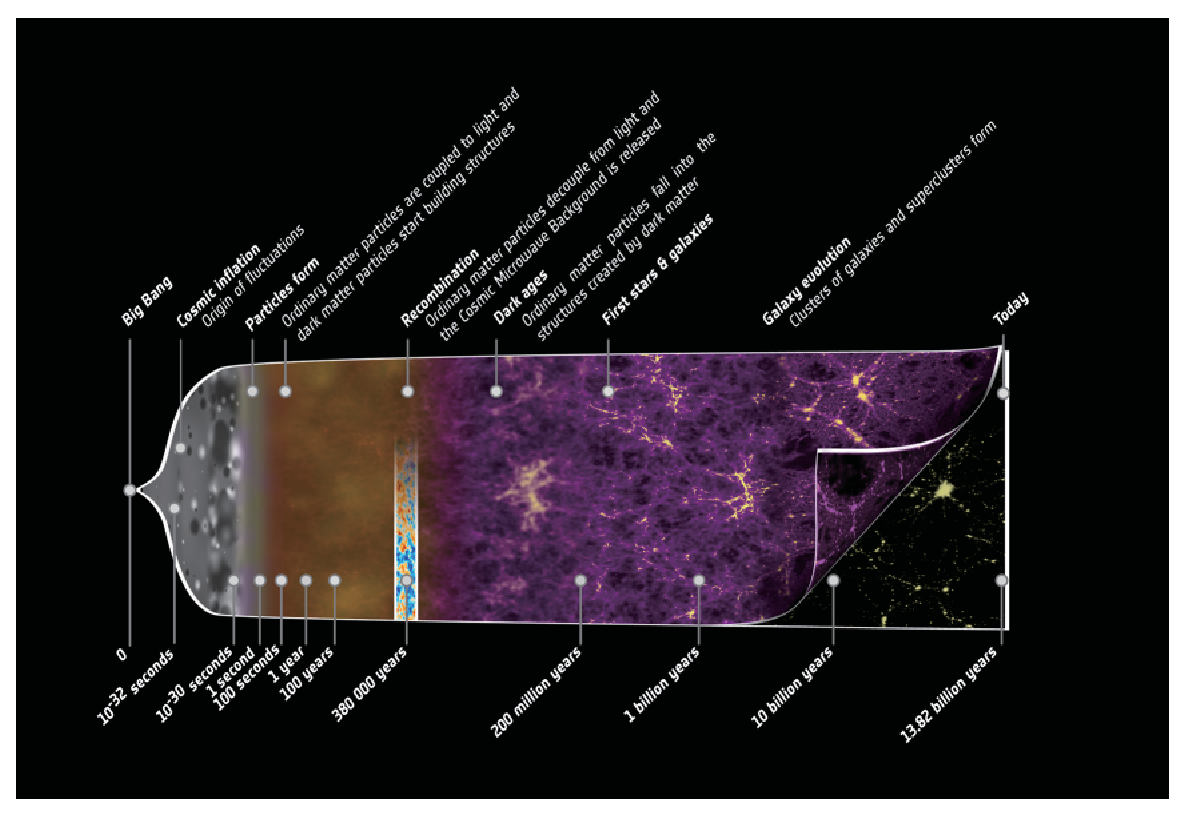
\includegraphics[width=0.8\linewidth]{cosmology/Planck_history_of_Universe_Crop_orig.eps} 
\caption{宇宙の構造進化の歴史(Planck web pageより)。}\label{fig:cosmo_history}
\end{center}
%\end{figure}
%%%%%%%%%%%%%%%%%%%%%%%%%%%%%%%%%%%%%%%%%%%%%%%%%%%%%%%%%%%%%%%%%%%%%%%%%%%%

%%%%%%%%%Figure%%%%%%%%%%%%%%%%%%%%%%%%%%%%%%%%%%%%%%%%%%%%%%%%%%%%%%%%%%%%%
%\begin{figure}[t]
 \begin{minipage}{0.6\hsize}
 \begin{center}
   \vspace{15pt}
   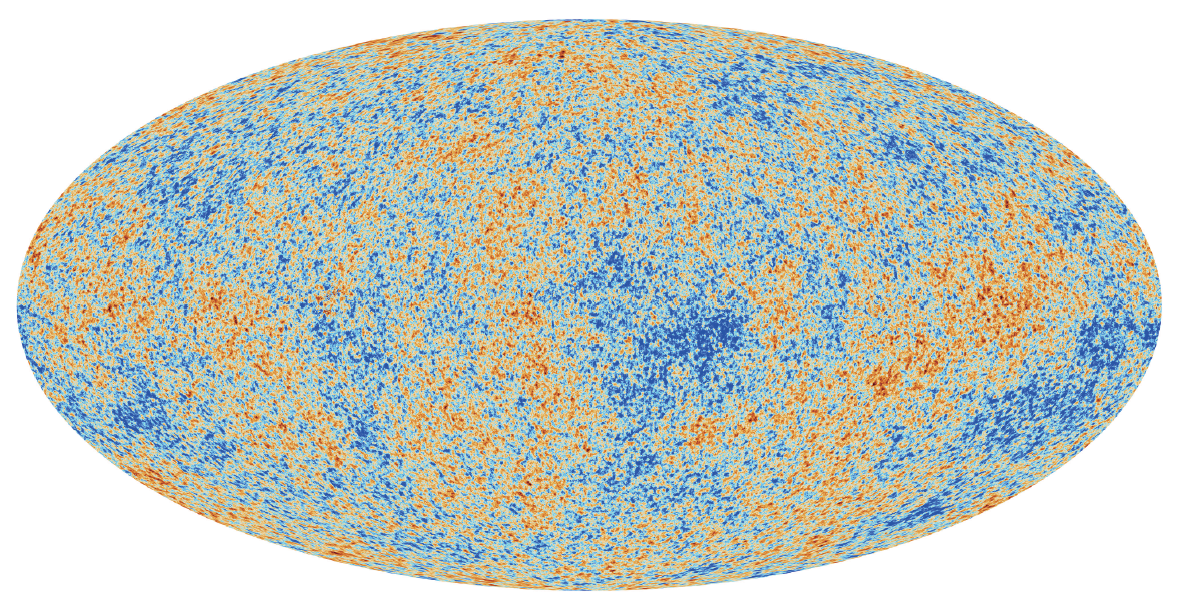
\includegraphics[width=0.7\linewidth]{cosmology/Planck_CMB_Mollweide_4k_2.eps} 
   \vspace{10pt}
   \caption{PlanckによるCMB温度揺らぎの全天マップ(Planck web pageより)}\label{fig:Planck_CMB}
 \end{center}
 \end{minipage}
 \begin{minipage}{0.4\hsize}
 \begin{center}
   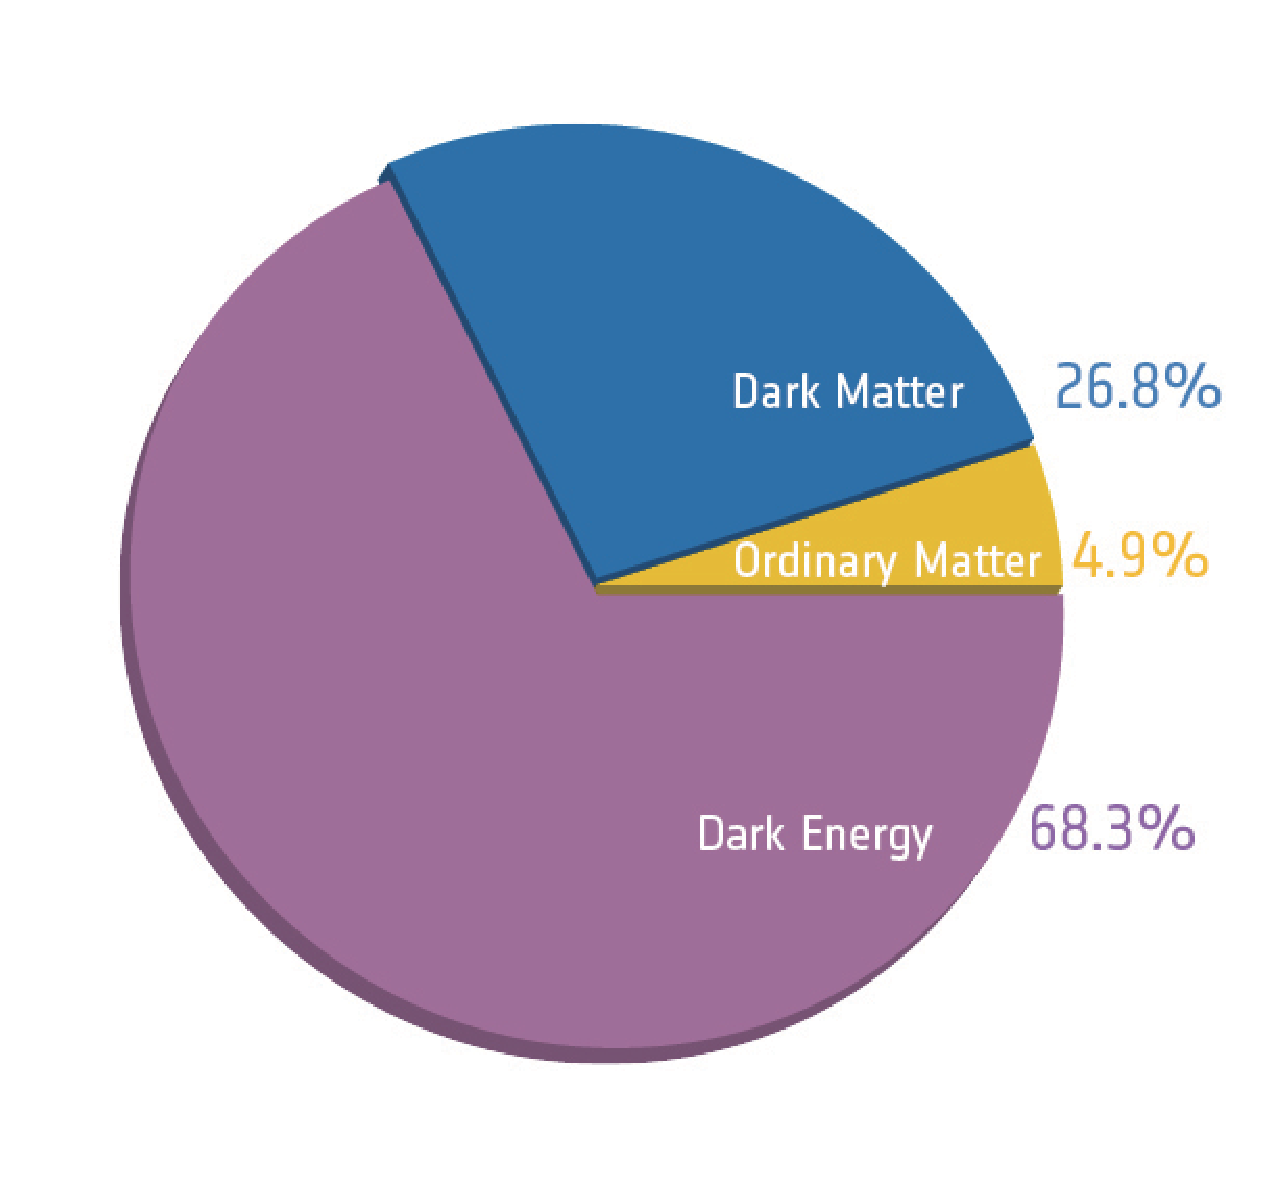
\includegraphics[width=0.8\linewidth]{cosmology/component_univ.eps} 
  \vspace{-15pt}
  \caption{宇宙の構成成分(Planck web pageより)。}\label{fig:component}  
 \end{center}
 \end{minipage}
\end{figure}
%%%%%%%%%%%%%%%%%%%%%%%%%%%%%%%%%%%%%%%%%%%%%%%%%%%%%%%%%%%%%%%%%%%%%%%%%%%%

宇宙論とは、宇宙全体やその内部に存在する構造物が、どのように形成されそして発展してきたのかについて、科学的手法を用いて理論的・観測的に解明していく学問である(図~\ref{fig:cosmo_history})。特に近年の観測技術の発達により、標準的な宇宙モデルはほぼ確立しており、それは次のようなものである。

まず、大局的なスケール(超銀河団を超えるスケール、約$100$Mpc以上)で宇宙を平均して見た場合、特別な場所は存在せず(一様性)、また特別な方向も存在しない(等方性)という一様等方宇宙モデルを採用している。現在のところ、このモデルが成り立っていないという確実な証拠は存在しない。さらに、宇宙内部の構成物についても、ビッグバン後約$38$万年頃に原子が形成され光が直進できるようになった時期の残光である宇宙マイクロ波背景放射(Cosmic Microwave Background radiation : CMB)の精密観測が行われたことにより(図\ref{fig:Planck_CMB})、このモデルの妥当性が確認されている。最新のCMB観測衛星Planck~\citep{Ade:2013zuv}の観測結果によると、通常の物質を構成するバリオンの量は、宇宙全体の約$5$\%程度に過ぎず、約$27$\%がほぼ重力相互作用しか行わない冷たい暗黒物質(cold dark matter)で構成され、さらに約$68$\% が宇宙の膨張を加速させる原因となる正体不明のエネルギー(暗黒エネルギー:dark energy)であるということが分かっている(図~\ref{fig:component})。またこのモデルでは一定の空間曲率が許されているが、CMBの観測からこの曲率は非常に小さく制限されており、この宇宙は平坦な宇宙であるということが判明している。典型的な宇宙論パラメータを表\ref{cosmological parameters1}, \ref{cosmological parameters2}に示す。

このように一様等方宇宙モデルは、観測を非常に良く説明するモデルであるが、そもそもなぜこのような条件の宇宙が生じたのかという疑問が生じてくる。その疑問に対し説明を与える最も有力なモデルが、宇宙初期における指数関数的急膨張(インフレーション)を仮定するモデルである。このインフレーションモデルでは、宇宙初期の光速を超える急膨張によって、当初因果関係を持っていた小さな領域を現在観測可能な範囲(宇宙の地平線)を超えて拡大することにより、非常に一様で等方な宇宙を実現することができる。またこの膨張によって、曲率は均されて小さくなり、非常に平坦な宇宙が実現する。さらにインフレーションモデルでは、インフレーションを生じさせる場としてインフラトンという場を仮定するが、その場の量子的な揺らぎから、銀河などの大規模構造の種となるわずかな密度揺らぎを生成することも可能にしている。

以上が現在標準的な宇宙モデルであるが、その上で今後解明を目指すべき重要な問題としては、次のようなものを挙げることができる:
(i) インフレーションモデルの検証、
(ii) 暗黒エネルギーの性質の解明及び修正重力理論の可能性の検証、
(iii) 暗黒物質の正体の特定。
以下で、これらの問題についての解説及びその観測的な制限について順に説明していく。

%\vspace{10pt}


%TTTTTTTTTTTTTTTTTTTTTTTTTTTTTTTTTTTTTTTTTTTTTTTTTTTTTTTTTTTTTTTTTTTTTTTTT%
\begin{center}
\begin{table}[t]
\caption{
標準的な宇宙論($\Lambda$CDM模型)におけるパラメータおよび$68\%$ C.L.エラー~\citep{Ade:2013zuv}。
}
\begin{center}
 \vspace{15pt}
\begin{tabular}{ccc} \hline \hline 
宇宙論パラメータ & 値 & 定義 \\ 
\hline 
$\Omega_{\rm b}h^2$ & $0.02214\pm 0.00024$ & 現在のバリオン密度\\
$\Omega_{\rm c}h^2$& $0.1187\pm 0.0017$ & 現在の冷たい暗黒物質密度\\
$\tau$ & $0.092\pm 0.013$ & 再電離によるトムソン散乱の光学的厚さ\\
$\ln (10^9 A_{\rm s})$ & $3.091\pm 0.025$ & 原始曲率揺らぎパワースペクトルの振幅\\
$n_{\rm s}$ & $0.9608\pm 0.0054$ & 原始曲率揺らぎパワースペクトルの冪指数\\
%\hline
$H_0=100h$ & $67.80\pm 0.77$ & 現在のハッブル定数 $[{\rm km}/{\rm s}/{\rm Mpc}]$\\
$\Omega_\Lambda$ & $0.692\pm 0.010$ & 現在の暗黒エネルギー密度\\
\hline
\hline 
\end{tabular}
\end{center}
\label{cosmological parameters1}
\end{table} 
\end{center}
%TTTTTTTTTTTTTTTTTTTTTTTTTTTTTTTTTTTTTTTTTTTTTTTTTTTTTTTTTTTTTTTTTTTTTTTTT%


%%%%%%%インフレーション関係%%%%%%%%%%%%%%%%%%%%%%%%%%%%%%%%%%%%%%%%%%%%%%%%%
\paragraph{(i) インフレーションモデルの検証}
%まず始めに、インフレーションモデルの検証方法について説明していく。
%
インフレーションモデルの検証において最も基本的な方法は、宇宙の密度揺らぎの測定である。これまで述べたように、インフラトンの量子揺らぎは最終的に密度揺らぎの起源となるが、この揺らぎはインフレーションのモデルの違いによって、特徴のある空間スケール依存性を示す。よって、その特徴を観測的に捉えることが、各インフレーションモデルを制限していく上で非常に有効な手段となる。

またインフレーションで生成される密度揺らぎはほぼガウス分布に従うことが知られているが、各モデルによってガウス分布からの微小なズレの程度(原始非ガウス性)が異なっている。そのため、この原始非ガウス性を測定することもこのモデルを制限する非常に有効な方法の一つである。
インフレーションの一般的なモデルでは、確率分布として様々な非ガウス性を持つ原始揺らぎを生成しうる。
原始揺らぎのガウス分布からのズレを表す最も便利な方法として、重力ポテンシャル$\Phi$が
ランダムガウス場$\phi$の線形項と2次の補正の和で
\begin{align}
	\Phi =\phi +f_{\rm NL}\left(\phi^2 -\langle\phi^2\rangle\right)
	\,.\label{eq:fNL def}
\end{align}
と書かれる場合を考える。
ここで、$f_{\rm NL}$は非線形パラメータと呼ばれる定数であり、$\langle\cdots\rangle$はアンサンブル平均を表す。
この場合、その統計的性質はパワースペクトルだけでは記述できず、
バイスペクトルのような高次のモーメントが必要になる。
異なるインフレーション模型は異なるバイスペクトルの形を予言することから、この探求により
インフレーションの物理について深い理解を得ることができる。
これまでCMBの精密な観測により、インフレーションの物理に対して精度よく制限がなされている(\ref{cosmology.s1.ss2}節)。
特に、Planck衛星による観測~\citep{Ade:2013ydc}によれば、非線形パラメータは$f_{\rm NL}=2.7\pm 5.8$となる制限が得られており、$f_{\rm NL}>10$となるような比較的大きな非ガウス性を生成するモデルや、モデル内のパラメータを制限することに成功している。
後述するように、銀河サーベイからも原始非ガウス性を探査することができる。
しかし、未知の系統誤差の影響により、現在までの制限は$\sigma (f_{\rm NL})\approx 50$程度に留まっている\citep{Ho:2013lda,Giannantonio:2013uqa}。

加えて、インフレーションの検証に非常に重要な観測として、インフレーション起源の原始重力波の観測が挙げられる。この原始重力波は、インフレーション中に重力場の量子揺らぎから生成されたものであり、その振幅はインフレーションのエネルギースケールと直接関係づくことが知られている。そのため、もしこの原始重力波を観測できれば、地上の加速器実験ではとても到達できない、
%ほど大きなエネルギーのスケールである
インフレーションの生じた超高エネルギーの物理の情報を直接知ることができるのである。

%現在、Planck衛星によるCMB温度揺らぎの観測から揺らぎのスケール依存性や原始重力波の強い制限が得られており~\citep{Ade:2013uln}、今後はより精密なCMB偏光の観測や、広い範囲の銀河サーベイ、または再電離の時期の水素が発する21cm線の観測によって、更に高い精度でインフレーションモデルの検証が行えると期待される。
%制限が得られると期待されている。
%また
%原始重力波については、
%その原始重力波の振幅が比較的大きなものであれば、
%将来の宇宙重力波干渉計を用いれば、原始重力波のスペクトルを直接観測できる可能性さえ存在している。


%TTTTTTTTTTTTTTTTTTTTTTTTTTTTTTTTTTTTTTTTTTTTTTTTTTTTTTTTTTTTTTTTTTTTTTTTT%
\begin{center}
\begin{table}[t]
\caption{
標準宇宙論に非標準的な$1$パラメータを加えた場合の$95\%$ C.L.エラー~\citep{Ade:2013zuv}。
}
\begin{center}
% \vspace{15pt}
\begin{tabular}{ccc} \hline \hline 
宇宙論パラメータ & 値 & 定義 \\ 
\hline 
$r$ & $<0.111$ & 原始重力波揺らぎパワースペクトルの振幅\\
$w$ & $-1.13
   \begin{array}{l}
      +0.23 \\
      -0.25
    \end{array}$
& 暗黒エネルギーの状態方程式\\
$\Omega_{\rm K}$ & $-0.0005
   \begin{array}{l}
      +0.0065 \\
      -0.0066
    \end{array}$
& 現在の空間曲率密度\\
$\frac{{\rm d}n_{\rm s}}{{\rm d}\ln k}$ & $-0.014
   \begin{array}{l}
      +0.016 \\
      -0.017
    \end{array}$
& 原始曲率揺らぎパワースペクトルの冪指数のランニング \\
$\sum m_\nu\,[{\rm eV}]$ & $<0.230$ & ニュートリノ質量和 \\
$N_{\rm eff}$ & $3.30
   \begin{array}{l}
      +0.54 \\
      -0.51
    \end{array}$
& ニュートリノの実効的な自由度の数\\
\hline
\hline 
\end{tabular}
\end{center}
\label{cosmological parameters2}
\end{table} 
\end{center}
%TTTTTTTTTTTTTTTTTTTTTTTTTTTTTTTTTTTTTTTTTTTTTTTTTTTTTTTTTTTTTTTTTTTTTTTTT%
%%%%%%%暗黒エネルギー関係%%%%%%%%%%%%%%%%%%%%%%%%%%%%%%%%%%%%%%%%%%%%%%%%%%%
\paragraph{(ii) 暗黒エネルギーの性質の解明及び修正重力理論の可能性の検証}
%%%%%%%%%%%%%%%%%%%%%%%%%%%%%%%%%%%%%%%%%%%%%%%%%%%%%%%%%%%%%%%%%%%%%%%%%%%%
%次に暗黒エネルギーの問題とについて説明していく。
%
宇宙の加速膨張の原因となるエネルギーを一般に暗黒エネルギーと呼ぶが、その存在が決定的になったのは、1990年代末のIa型超新星を用いた宇宙膨張の観測以降である~\citep{Riess:1998cb,Perlmutter:1998np}。
それらの観測により、観測された超新星の見かけの光度が、減速膨張宇宙の場合と比べて暗いという事実が発見された。
これは同じ後退速度で運動する、もしくは同じ赤方偏移を示す超新星までの距離が減速しているときに比べて相対的に大きいことを意味する。
このことから、宇宙が加速膨張しているということが判明した。

この暗黒エネルギーの最も単純な候補は、時間変化しない一定密度のエネルギー(宇宙定数)であり、そのようなエネルギーとして量子場の真空のエネルギーが考えられている。しかし、この場合、理論的に推定される真空のエネルギー密度は、観測された暗黒エネルギーの密度より120桁以上も大きな値となってしまい、この様な微小な真空のエネルギーを自然に説明することは非常に難しい。

そのため、加速膨張がそのような真空のエネルギー起源ではなく、何等かの加速膨張の原因となる新しい場を導入するモデル(クインテッセンス等)も数多く提案されている。
さらに一般相対性理論自体を修正することにより加速膨張を説明するというアプローチも存在し、それらは一般に修正重力理論と呼ばれている。
一般相対論は、重力の効果が弱い実験室や太陽系スケールでは既に非常に厳しい制限がなされているが、重力が
重要になりえる宇宙論的な大スケールでは大きくずれている可能性がある。
観測的な制限を回避しうる模型がいくつか提案されており、その中で有名な模型としては
$f(R)$重力理論、DGPブレーンワールド模型、スカラーテンソル理論、有質量重力理論等がある。
また一様等方宇宙モデルを修正した非一様宇宙モデルによって観測を説明するという方向も考えられている。

これら宇宙定数以外のモデルの場合、暗黒エネルギーの密度は一般に時間変化することから、この影響を観測することで
宇宙定数の場合と区別することが可能である。
特に、暗黒エネルギーのエネルギー密度$\rho$および圧力$P$を用いて作られる状態方程式パラメータ
\begin{align}
	w=\frac{P}{\rho}\,,
	\label{eq:DE EOS def}
\end{align}
を検証することが行われている。
多くの場合、$w$を定数として扱い制限を行ってきた(表\ref{cosmological parameters2}参照)。
状態方程式パラメータの時間進化を特徴付ける代表的な方法として、
\begin{align}
	w(z)=w_0+w_a\,\frac{z}{1+z}
	\,,
	\label{eq:DE EOS}
\end{align}
となる二つの定数$w_0,w_a$を導入する手法も行われている。
宇宙項が暗黒エネルギーだった場合、その状態方程式$w$は厳密に$-1$となるため、$(w_0,w_a)=(-1,0)$に対応する。
修正重力理論の場合には、一般的に$w$が時間進化することから$w_a$が非自明な値をとり得る。
これらは、宇宙膨張が密度揺らぎの成長に与える影響、特にバリオン音響振動(Baryon Acoustic Oscillation; BAO)
および赤方偏移空間歪み(Redshift Space Distortion; RSD)と呼ばれる効果を銀河の赤方偏移サーベイによって
観測することで知ることができる(\ref{cosmology.s1.ss1-2}節)。
現在の所、CMBと超新星の観測及びBAOの観測を組み合わせることにより、
暗黒エネルギーの状態方程式パラメータに対し
$w_0=-1.04
   \begin{array}{l}
      +0.72 \\
      -0.69
	\end{array}$
および$w_a<1.32$なる制限が得られているが、
有意な宇宙定数からのズレは今のところ観測されてはいない~\citep{Ade:2013zuv}。そのため今後は、より広い赤方偏移の観測を行うことにより、本当に暗黒エネルギーが宇宙定数であるのか、それとも厳密な宇宙定数の場合とは違いがあるのかについて、より精密に測定していくことが宇宙論における重要な目標となっている。


%%%%%%%暗黒物質%%%%%%%%%%%%%%%%%%%%%%%%%%%%%%%%%%%%%%%%%%%%%%%%%%%%%%%%%%%%
\paragraph{(iii) 暗黒物質の正体の特定}
%%%%%%%%%%%%%%%%%%%%%%%%%%%%%%%%%%%%%%%%%%%%%%%%%%%%%%%%%%%%%%%%%%%%%%%%%%%%
最後に正体は不明ながらも、現在その存在はほぼ確実視されている冷たい暗黒物質とその観測可能性について説明していく。まず冷たい暗黒物質とは、運動エネルギーが質量エネルギーより小さい暗黒物質のことであり、逆に運動エネルギーが大きな暗黒物質のことを熱い暗黒物質と呼ぶ。熱い暗黒物質は自身の自由運動のために、小スケールの密度揺らぎが均されて消されてしまい、観測されている密度揺らぎを正しく説明することができない。そのため、暗黒物質は冷たい暗黒物質がほとんどを占めていると考えられている。

通常の物質とはほぼ相互作用せず、重力によってのみ相互作用する暗黒物質の存在は、1930年代には銀河団の解析から既に示唆されており、また1970年代には銀河の回転曲線の観測から銀河は光を放っている円盤部分よりも質量を担う領域が大きく広がっており、むしろそちらが銀河の質量の大部分を占めているということが判明していた。

そのため、その正体を突き止めることが現在の宇宙論における目標の一つとなっている。暗黒物質の正体を探る方法としては、暗黒物質がわずかに行う可能性のある通常の物質との相互作用を検出する直接検出実験
や、暗黒物質が対消滅や崩壊をする際に生成されるガンマ線や高エネルギーの粒子を観測する間接検出実験が多数行われている状況である。
また、現在においては、銀河サーベイにおける弱重力レンズ効果(\ref{cosmology.s1.ss1-2}節)を用いることで、
前景にある暗黒物質量を推定することができることから暗黒物質の空間分布を観測から探ることも広く行われている。

\subsection{宇宙論的観測手法}\label{cosmology.s1.ss1-2}

この節では、銀河サーベイを用いた代表的な観測手法についていくつか簡単に触れておくことにする。
まず既に言及したBAOについて説明する。
バリオン音響振動とは宇宙の再結合以前に光子とバリオンがトムソン散乱とクーロン相互作用を
通じて混合流体として存在していた時期の音波振動と、再結合後に音波振動が光子から
脱結合したバリオンとダークマターの重力相互作用を通じて宇宙大規模構造に反映された振動パターンを指す。
後者のBAO振動パターンのスケールは、音響ホライズンと呼ばれる混合流体の音波が再結合までの宇宙年齢をかけて進む距離
$r_{\rm s}$で与えられ、密度揺らぎの相関関数に特徴的なピークを残す効果として観測される(図~\ref{fig:BOSS_BAO})。
再結合時から現在に至るまで不変であるため宇宙の大規模構造を測定する際の距離指標として使うことが可能である。
そのため、宇宙の大規模構造の観測でBAOを検出することによって宇宙の空間的な幾何学や膨張の履歴を小さな系統誤差で
導くことが可能で、ダークエネルギーの物理的性質、一般相対論的な重力理論の検証などの宇宙に関する物理学の基本的問
題を調べる手段となりうる。


%%%%%%%%%Figure%%%%%%%%%%%%%%%%%%%%%%%%%%%%%%%%%%%%%%%%%%%%%%%%%%%%%%%%%%%%%
\begin{figure}[t]
 \begin{minipage}{0.5\hsize}
 \begin{center}
   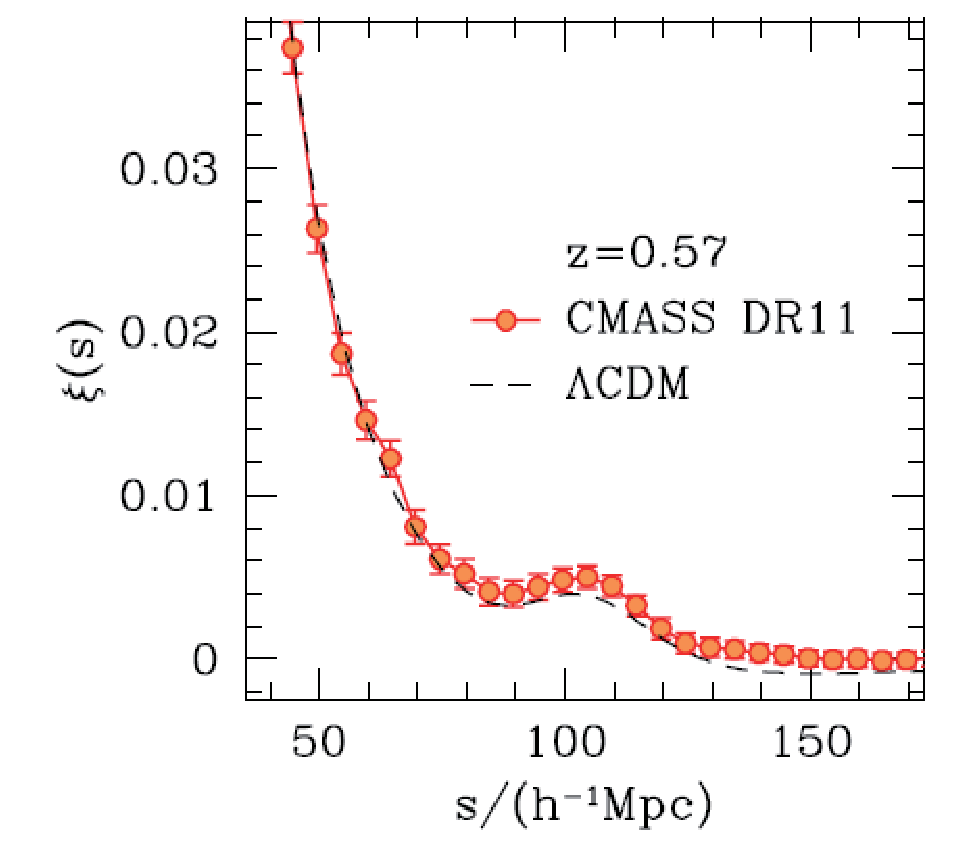
\includegraphics[width=0.95\linewidth]{cosmology/SDSS_BOSS_DR11_BAO.eps}   
   \caption{SDSS-III BOSSサーベイ(DR11)による角度平均した銀河の相関関数$\xi$~\citep{Sanchez:2013tga}。
            横軸は距離のスケールを表し、$100{\rm h}^{-1}{\rm Mpc}$付近にバリオン音響振動による
            ピークが見える。なお$\Lambda$CDMとは標準宇宙モデルのことである。}\label{fig:BOSS_BAO}
 \end{center}
 \end{minipage}
 \hspace{5pt}
 \begin{minipage}{0.5\hsize}
 \begin{center}\vspace{-10pt}
   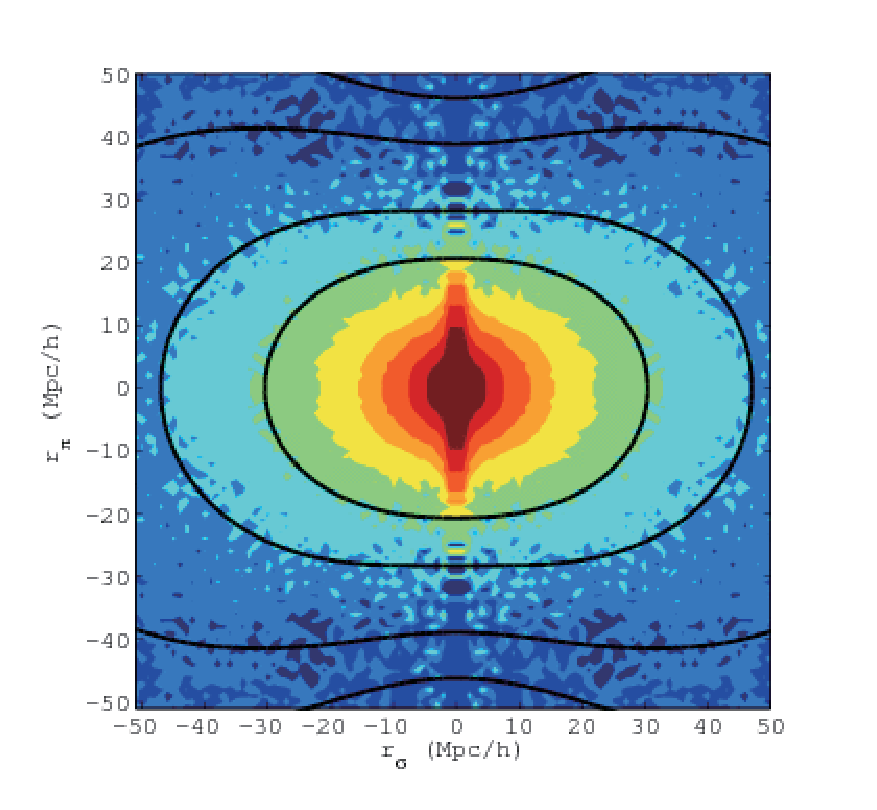
\includegraphics[width=0.95\linewidth]{cosmology/butterfly_colour_smallerscales.eps} 
   %\vspace{10pt}
   \caption{SDSS-III BOSSサーベイ(DR9)による、銀河の相関関数(赤いほど相関関数が大きい)~\citep{Reid:2012sw}。
           縦軸は視線方向、横軸は天球面上での距離スケールである。
           この縦方向と横方向における歪みが、赤方偏移空間歪みである。
           }\label{fig:BOSS_RSD}  
 \end{center}
 \end{minipage}
\end{figure}
%%%%%%%%%%%%%%%%%%%%%%%%%%%%%%%%%%%%%%%%%%%%%%%%%%%%%%%%%%%%%%%%%%%%%%%%%%%%

加えて、銀河の相関関数の非等方性として観測されるRSDも非常に有用な手法として
盛んに利用されている。赤方偏移空間歪みとは、個々の銀河の固有速度によって生じた赤方偏移による効果で、
たとえ実空間における銀河の分布が等方であっても、実際に観測される赤方偏移空間上では非等方な揺らぎとなってしまうことから発生する(図~\ref{fig:BOSS_RSD})。この固有速度の影響は、密度揺らぎの成長率と関係づくため、その成長に対する暗黒エネルギーの影響を調べることに利用することができる。

最後に、弱重力レンズ効果を利用した方法を説明する。
重力レンズ効果は、サーベイ対象の銀河からの光が経路上の物質による重力によって経路が直線からズレることで発生する。
その中でも弱重力レンズ効果とは、物質の重力によって発生する重力レンズ効果の内、
像の歪みが小さいために単独の観測対象を見ているだけでは
その影響が分からないもののことを呼ぶ。
したがってこの弱重力レンズ効果は、多数の観測対象を統計的に処理することで、
初めてその効果を測定することが可能となる。
%
この弱重力レンズ効果は宇宙の物質分布つまり密度揺らぎの情報を保持しており、
暗黒物質のエネルギー密度や暗黒エネルギーが密度揺らぎの成長に与える影響などについて、
詳細に調べるために利用することができる。

%%%%%%%%%%%%%%%%%%%%%%%%%%%%%%%%%%%%%%%%%%%%%%%%%%%
\vspace{15pt}

%%%%%%%まとめ%%%%%%%%%%%%%%%%%%%%%%%%%%%%%%%%%%%%%%

以上の様に、宇宙論における未解決問題であるインフレーションの検証、暗黒エネルギーおよび暗黒物質の正体の特定に向け、
様々な観測手法を用いることで宇宙論研究が行われている。
ここまで挙げた観測手法による宇宙論は、これまではほとんど光赤外観測によって推進されてきた。
将来観測(電波以外の波長については次節参照)により、これらの理解は格段に進歩することが予想される。
しかし、今後はSKAが登場することで電波によりこれらの観測を行うことが可能になり、電波観測によるこれまでにない規模・精度の
宇宙論を行うことができるようになる。
これにより、理論・観測両方面における宇宙論分野の更なる発展が期待される。

\subsection{他波長の将来計画}\label{cosmology.s1.ss2}

\subsubsection{マイクロ波背景放射}
これまで、COBEによる黒体輻射スペクトルの精密測定、地平線を超えた温度揺らぎの検出に始まり、DASIによるEモード偏光の検出~\citep{Kovac:2002fg}, WMAP衛星~\citep{Bennett:2012zja}, Planck衛星~\citep{Ade:2013zuv}による温度揺らぎの精密観測による宇宙論パラメタの決定、最近ではSPTPol~\citep{Hanson:2013hsb}, PolarBear~\citep{Ade:2013hjl}両実験による重力レンズ由来のBモード偏光の検出、さらにはBICEP2実験による重力波由来のBモード偏光の検出~\citep{Ade:2014xna}と、CMB実験はここ10年で急速な進展を遂げている。2014年末のPlanck衛星の偏光揺らぎの観測結果の発表をもって線形段階の密度揺らぎに由来するCMB温度揺らぎ・偏光揺らぎの観測は一段落を迎えることになる。%このPLANCKの結果次第でもあるが、その後の
今後のCMBの観測的研究の方向は大きく以下の4つが考えられる。
(観測計画リストは\ref{table:CMB future plan}参照)


\paragraph{重力波由来のBモード偏光スペクトルの詳細観測}
BICEP2によって報告されたBモード偏光検出については主要な観測が$1$周波数帯のみでしか行われておらず、前景放射のもれこみの問題が指摘されている\citep{Flauger:2014qra,Mortonson:2014bja}。Planckの複数の周波数帯による偏光観測により前景放射の情報が得られることが期待されているが~\citep{Adam:2014bub}、もしBICEP2の検出したシグナルが前景放射によるものだった場合、これまで以上に感度を上げた観測が必要となる。また、インフレーション由来の重力波であることを結論付けるためには、再イオン化によるバンプや整合性条件のチェックなど、広いスケールに渡ってスペクトルを観測する必要があり(例えば\citep{Dodelson:2014exa})、大角度スケールの観測に特化した地上観測や、衛星観測が必要になる。


\paragraph{重力レンズ由来のBモード偏光観測}
CMB弱重力レンズ効果は、宇宙晴れ上がり時の温度・偏光揺らぎの分布が、手前にある大規模構造による重力ポテンシャルによって歪められることによって発生する。特に密度揺らぎ起源であるEモードがレンズ効果によりBモードに変換されるが、このBモードは小スケールで他からのシグナルを卓越するため、重力ポテンシャルを再構築するのに適している\citep{Okamoto:2003zw,Hirata:2003ka}。重力レンズ効果によって推定される大規模構造は宇宙に存在する物質と重力の情報を含むため、例えばニュートリノ質量の精密測定や重力理論の検証などに用いることができる。


\paragraph{スニヤエフ・ゼルドビッチ(Sunyaev-Zel'dovich; SZ)効果}
大規模構造に付随する高温プラズマ(主に銀河団)はCMB光子を電子の熱運動によって逆コンプトン散乱することにより、CMBの黒体放射を歪ませる(熱的SZ)。この歪みの大きさは高温ガスの内部エネルギーに比例するため、重力ポテンシャルすなわち銀河団の質量のよい指標になる。また、この歪みは高周波側では温度の上昇、低周波側では温度の下降として観測され、温度揺らぎの観測からも検出することができる。一方、宇宙の再イオン化期に生成されるイオン化領域によるコンプトン散乱はその領域の特異速度に依存したドップラー効果により新たな温度揺らぎを生み出し(動的SZ)この効果を観測することにより、宇宙再イオン化期の情報(再イオン化開始時刻や時間など)を得ることが期待できる。


\paragraph{スペクトル歪みの詳細観測}
角度揺らぎとは別の方向性として、CMBのプランク分布からのずれの詳細な観測が計画・議論されている。宇宙初期における熱浴への熱流入は時期によって$\mu$歪み・$y$歪みを引き起こし、この歪みを詳細に観測することにより初期宇宙での物理過程を調べることができる。物理過程には、スニヤエフ・ゼルドビッチ効果の他に例えば粘性散逸による加熱や、ダークマターの崩壊、初期磁場の散逸などがある~\citep{Tashiro:2014pga}。


\begin{table}
 \centering
 \begin{tabular}{c|l|cccc}\hline\hline
  種類 &  \hspace{2zw}計画名\hspace{2zw} & 重力波 & 重力レンズ & \hspace{0.5zw}SZ\hspace{0.5zw} & スペクトル歪み \\\hline
  \multirow{4}{*}{人工衛星}
  & COrE+ & \checkmark & \checkmark & \checkmark \\\cline{2-6}
  & EPIC-IM & \checkmark & \checkmark & \checkmark & \\\cline{2-6}
  & LiteBIRD & \checkmark & & & \\\cline{2-6}
  & PIXIE & \checkmark & & & \checkmark \\\hline
  \multirow{5}{*}{バルーン}
  & EBEX* & \multirow{2}{*}{\checkmark} & & & \\
  & EBEX6K & & & & \\\cline{2-6}
  & LSPE & \checkmark & & & \\\cline{2-6} 
  & PIPER* & \checkmark & & & \\\cline{2-6} 
  & \textsc{Spider}* & \checkmark & & & \\\hline
  \multirow{17}{*}{地上}
  & ABS* & \checkmark & & & \\\cline{2-6}
  & ACTPol* & \multirow{2}{*}{\checkmark} & \multirow{2}{*}{\checkmark} & \multirow{2}{*}{\checkmark} & \\
  & AdvACTPol* & & & & \\\cline{2-6}
  & B-Machine* & \checkmark & & & \\\cline{2-6}
  & CLASS* & \checkmark & & & \\\cline{2-6}
  & GLP & \checkmark & & & \\\cline{2-6}
  & GroundBIRD & \checkmark & & & \\\cline{2-6}
  & Keck array* & \multirow{2}{*}{\checkmark} & & & \\
  & BICEP3* & & & & \\\cline{2-6}
  & MuSE & \checkmark & & & \\\cline{2-6}
  & \textsc{Polarbear}* & \multirow{3}{*}{\checkmark} & \multirow{3}{*}{\checkmark} & & \\
  & \textsc{Polarbear-2}* & & & & \\
  & Simons Array* & & & & \\\cline{2-6}
  & QUBIC* & \checkmark & & & \\\cline{2-6}
  & QUIJOTE* & \checkmark & & & \\\cline{2-6}
  & SPTpol* & \multirow{2}{*}{\checkmark} & \multirow{2}{*}{\checkmark} & \multirow{2}{*}{\checkmark} & \\
  & SPT-3G* & & & & \\\hline\hline
\end{tabular}
\caption{各CMB観測に関する星取表。*印は観測予定または観測中のもの。
ただし、重力波に関しては各実験が「low-$\ell$をターゲットにしている」「low-$\ell$を観測出来る」と明記しているもの、
重力レンズに関しては独自に重力レンズ角度パワースペクトルを評価できるだけチェックマーク( $\checkmark$ )を付けている。
監修:茅根氏}
\label{table:CMB future plan}
\end{table}



\subsubsection{光赤外}

宇宙論を主なターゲットにした光赤外サーベイは数多く計画されている。主要なアプローチとしては、弱い重力レンズの統計、銀河などの天体の空間分布の相関関数によるバリオン音響振動や赤方偏移空間歪みの効果、Ia型超新星爆発などが用いられる。観測装置としては地上望遠鏡と宇宙望遠鏡を使う方法に大別される。宇宙望遠鏡は大気の窓を越えてしか観測できない中間・遠赤外線の場合には地上では難しい高空間分解能や高感度を達成しうるという利点はあるが、一方で大口径の望遠鏡や超広視野の撮像装置、大掛かりな分光装置などを宇宙に打ち上げるのは非現実的であるので地上の大型望遠鏡も相補的な重要な役割を果たす。サーベイ観測には撮像サーベイと分光サーベイがあり前者は主に重力レンズやIa型超新星爆発、後者は主に銀河相関関数を用いた宇宙論を目指しこれらも相補的である。

撮像サーベイで$2020$年頃までの主力となるのは、すばる$8$m望遠鏡を用いた日本の Hyper Suprime-Cam (HSC) サーベイとアメリカが主導するチリの4m望遠鏡を使ったDark Energy Survey (DES) である。HSCは$1400$~deg$^2$の領域を$r\sim 26$等の深さで観測するのに対して、DESは$5000$~deg$^2$の領域を$r\sim 25$等とやや浅く観測していく。両者ともサーベイ観測を開始したばかりであり$5$年かけてサーベイを行っていく。

$2020$年以降に主力となる次世代サーベイはEuclid (Europian Space Agency (ESA))、WFIRST-AFTA (NASA)、Large Synoptic Survey Telescope (LSST; アメリカ) である。EuclidとWFIRST-AFTAは宇宙望遠鏡であり、地上からは感度が悪い近赤外での観測に重点がおかれている。また宇宙での観測は高空間分解能の画像が容易に得られるので弱い重力レンズで必須となる銀河の精確な形状測定の上で多くの利点がある。実際にEuclidは$15000$~deg$^2$の$r\sim25 $等の撮像データを用いた重力レンズ宇宙論を主なターゲットとしている。WFIRST-AFTAは多目的宇宙望遠鏡ではあるが$2000$~deg$^2$程度の領域をEuclidよりも深く観測し弱い重力レンズなどに用いることが予定されている。また遠方のIa型超新星爆発を狙った超新星サーベイも計画されている。LSSTはチリに$8$mの専用望遠鏡を設置しサーベイ観測を行う。LSSTは南天の$20000$~deg$^2$の領域を観測するが、その大きな特長としては時間変動の大規模なサーベイを行う点にある。具体的にはLSSTは一回の撮像で$r\sim 24$等の浅い観測を行い、この観測を数日おきに何度も繰り返し、最終的には同じ空の領域を何百回と観測し最終的な撮像データは$r\sim 27$等に達すると見積もられている。これにより時間変動する天体、例えば超新星爆発やクエーサーといった天体を全天規模で大量に発見することができ、時間変動天体に対する理解が圧倒的に進むであろうと期待されている。これに関しては東京大学で計画されているThe University of Tokyo Atacama Observatory (TAO)も重要な寄与をすると期待される。この大規模な時間変動を利用した宇宙論研究、たとえばIa型超新星爆発の統計解析や強い重力レンズの時間の遅れの研究などで大きな進歩が期待できる。

一方将来の分光サーベイとしては、Sloan Digital Sky Surveyの第四期サーベイの一つ Extended Baryon Oscillation Spectroscopic Survey (eBOSS; $2014$年開始)、すばる望遠鏡に取り付けられる予定の多天体分光器 Prime Focas Spectrograph (PFS; $2017$年頃以降)などがあり、$2020$年以降には地上4m望遠鏡に多天体分光器を取り付けるアメリカの計画 Dark Energy Spectroscopic Instrument (DESI) もある。またEuclidとWFIRST-AFTAの宇宙望遠鏡にもスリットレス分光機能が搭載され分光サーベイ観測を行う予定である。これらの分光サーベイの一番のターゲットはバリオン音響振動の観測による角径距離とハッブルパラメータの精密測定であり、これら将来計画により$0<z<3$の範囲で距離を1\%以下で測定しダークエネルギーの状態方程式に厳しい制限をつけることを目指す。

またこれらサーベイ観測と並んで、地上に$30$m級の大型望遠鏡を作る動きもある。アメリカや日本が主導する Thirty Meter Telescope (TMT)もその一つであり、ハワイに$30$m望遠鏡に設置し$2021$年稼働開始を目指している。ヨーロッパが主導するチリに$39$m望遠鏡を設置する European Extremely Large Telescope (E-ELT)、アメリカなどの同じくチリに$22$m望遠鏡を設置するGiant Magellan Telescope (GMT) も同時期の$2020$年頃の稼働を目指している。これらの大型望遠鏡は、暗い遠方銀河の分光観測による測光的赤方偏移の較正、遠方超新星爆発や強い重力レンズなどの宇宙論的に重要な天体の分光や補償光学を用いた高空間分解能撮像などの場面で活躍すると期待され、宇宙論研究にやはり重要な役割を果たす。



\subsubsection{X線}
X線観測による宇宙論の研究では、銀河団・銀河群の探査を行い、光赤外の観測による重力レンズ効果・電波観測によるSZ効果などから較正を行った推定質量を用いて銀河団・銀河群の質量関数と理論的なダークマターハローの質量関数を比較することで、宇宙論パラメータ・原始非ガウス性・重力理論などに制限を課すことが行われている。X線観測衛星のミッションは大きく分けて、銀河団・銀河群の大規模なカタログを作るsurvey型のミッションと、個々の銀河団を詳しく調べて推定質量の較正に役立てるobservatory型のミッションに分けられる。SKAが運用されるまでの今後$10$年間に計画されているX線観測衛星計画で、宇宙論的な文脈での研究が中心的なサイエンスを占めるものを以下に列挙する。
\begin{itemize}
\item ASTRO-H (日本・observatory型)\\
$2015$年秋に打ち上げ予定の日本のX線観測衛星で、世界で最初のTranslation Edge Sensor (TES)カロリメータを用いたX線分光装置 Soft X-ray Spectrograph (SXS) とCCDカメラSoft X-ray Imager (SXI) を用いた銀河団とその外縁部のX線観測が特徴的。
\item eROSITA on Spektr-RG (Russia, Germany・survey型)\\
ロシアとドイツが共同開発するSpektr-RGというX線観測衛星の観測装置の一つ。2014年Q3に打ち上げ予定だったが2015年に延期。有効面積の大きなX線望遠鏡とX線CCDの組み合わせで、X線での全天サーベイを行い銀河団とAGNのカタログを作成する予定。
\item DIOS (日本・observatory型)\\
ダークバリオンの大半を占めると考えられるWarm-Hot Intergalactic Medium (WHIM) 探査に特化したX線観測衛星。Diffuse Intergalactic Oxygen Surveyorの略。JAXA/ISASのイプシロンロケットを用いた小型科学衛星シリーズでの打ち上げを検討中。ASTRO-Hの$200$倍以上という非常に大きなグラプス(望遠鏡の有効面積と視野の積)を持つX線望遠鏡、TESカロリメータを用いた高いエネルギー分解能(5eV以下)のX線分光装置が特徴で$2020$年ごろの打ち上げを予定。
\item ATHENA (ESA)\\
ESAが計画中のX線観測衛星で$2028$年打ち上げ予定。eROSITAの更に$10$倍以上の有効面積を持つWide Field Imager (WFI)とTESカロリメータを用いた高いエネルギー分解能をもつX線分光器X-ray Integral Field Unit (X-IFU)を搭載し、これまでにない深いX線観測を行うことが可能になる。銀河団に関しては、赤方偏移が$1$を超える宇宙での銀河団や銀河群を内部構造も含めて観測する。また、再電離期程度の遠方宇宙までの銀河中心ブラックホールを観測することで、巨大ブラックホールの成長を理解することを目指している。
\end{itemize}




\subsection{SKA pathfinderによる宇宙論}\label{cosmology.s1.ss3}

以下、SKAのpathfinderによる宇宙論に関連したサーベイ計画をまとめておく。

\subsubsection{continuum survey}
\begin{itemize}
\item ASKAP EMU\\
正式名称はEvolutionary Map of the Universeで全天の75\%を$10~\mu{\rm Jy/beam~rms}$の感度、10-15 arcsecの角度分解能でサーベイし、約7千万個の銀河を観測する。$z=1$までのstar forming galaxyを観測できると期待されている。周波数帯は700-1800 MHz。
\item WODAN\\
正式名称はWesterbork Observations of the Deep APERTIF Northern-Skyで、WSRT (Westerbork Synthesis Radio Telescope)に配備されたphased array feed受信機であるAPERTIFを用いたサーベイである。ASKAPで観測できない全天の25\%の領域を$10~\mu{\rm Jy/beam~rms}$の感度、15 arcsecの角度分解能で観測する。
\item MeerKAT MIGHTEE\\
正式名称はMeerKAT International GigaHertz Tiered Extragalactic Exploration Survey。1.4 GHzでASKAP EMUやWODANに比べて狭い領域を深く観測する。
\item LOFAR\\
30-80 MHzと110-240 MHzの低周波で観測する。Tier 1, Tier 2, Tier 3の3つのサーベイフェイズがある。
\end{itemize}

\subsubsection{HI survey}

\begin{itemize}
\item ASKAP WALLABY\\
正式名称はWidefield ASKAP L-Band Legacy All-Sky Blind Surveyで全天の75\%を観測し$z=0.26$までの銀河を$500,000$個観測できる見込み。
\end{itemize}


